\hypertarget{predicting-crime}{%
\chapter{Predicting Crime}\label{predicting-crime}}

This chapter and the next make up a case study related to ``Machine
Bias'', an article published by ProPublica in 2016 (see
\url{https://www.propublica.org/article/machine-bias-risk-assessments-in-criminal-sentencing}).
The article explores the use of predictive algorithms in the criminal
justice system.

\begin{itemize}
\item
  In this chapter, we'll replicate the analysis described in the article
  and compute statistics that evaluate these algorithms, including
  accuracy, predictive value, false positive rate, and false negative
  rate.
\item
  In the next chapter, we'll review arguments presented in a response
  article published in the Washington Post. We'll compute and interpret
  calibration curves, and explore the trade-offs between predictive
  value and error rates.
\end{itemize}

\hypertarget{machine-bias}{%
\section{Machine Bias}\label{machine-bias}}

We'll start by replicating the analysis reported in ``Machine Bias'', by
Julia Angwin, Jeff Larson, Surya Mattu and Lauren Kirchner, and
published by ProPublica in May 2016.

This article is about a statistical tool called COMPAS which is used in
some criminal justice systems to inform decisions about which defendants
should be released on bail before trial, how long convicted defendants
should be imprisoned, and whether prisoners should be released on
probation (see \url{https://en.wikipedia.org/wiki/COMPAS_(software)}).

COMPAS uses information about defendants to generate a ``risk score''
which is intended to quantify the risk that the defendant would commit
another crime if released.

The authors of the ProPublica article used public data to assess the
accuracy of those risk scores. They explain:

\begin{quote}
We obtained the risk scores assigned to more than 7,000 people arrested
in Broward County, Florida, in 2013 and 2014 and checked to see how many
were charged with new crimes over the next two years, the same benchmark
used by the creators of the algorithm.
\end{quote}

In their notebook (see
\url{https://github.com/propublica/compas-analysis/blob/master/Compas\%20Analysis.ipynb}),
they explain in more detail:

\begin{quote}
We filtered the underlying data from Broward county to include only
those rows representing people who had either recidivated in two years,
or had at least two years outside of a correctional facility.

{[}\ldots{]}

Next, we sought to determine if a person had been charged with a new
crime subsequent to the crime for which they were COMPAS screened. We
did not count traffic tickets and some municipal ordinance violations as
recidivism. We did not count as recidivists people who were arrested for
failing to appear at their court hearings, or people who were later
charged with a crime that occurred prior to their COMPAS screening.
\end{quote}

If you are not familiar with the word ``recidivism'', it usually means a
tendency to relapse into criminal behavior. In this context, a person is
a ``recidivist'' if they are charged with another crime within two years
of release. However, note that there is a big difference between
\emph{committing} another crime and being \emph{charged} with another
crime. We will come back to this issue.

The authors of the ProPublica article use this data to evaluate how well
COMPAS predicts the risk that a defendant will be charged with another
crime within two years of their release.

Among their findings, they report:

\begin{quote}
\ldots{} the algorithm was somewhat more accurate than a coin flip. Of
those deemed likely to re-offend, 61 percent were arrested for any
subsequent crimes within two years.

\ldots{} In forecasting who would re-offend, the algorithm made mistakes
with Black and White defendants at roughly the same rate but in very
different ways.

\begin{itemize}
\item
  The formula was particularly likely to falsely flag Black defendants
  as future criminals, wrongly labeling them this way at almost twice
  the rate as White defendants.
\item
  White defendants were mislabeled as low risk more often than Black
  defendants.
\end{itemize}
\end{quote}

This discrepancy suggests that the use of COMPAS in the criminal justice
system is racially biased.

Since the ProPublica article was published, it has been widely discussed
in the media, and a number of researchers have published responses. In
order to evaluate the original article and the responses it provoked,
there are some technical issues you need to understand. My goal is to
help you analyze the arguments and interpret the statistics they are
based on.

\hypertarget{replicating-the-analysis}{%
\section{Replicating the Analysis}\label{replicating-the-analysis}}

The data used in ``Machine Bias'' is available from
\url{https://github.com/propublica/compas-analysis}.

We can use Pandas to read the file and make a
\passthrough{\lstinline!DataFrame!}.

\begin{lstlisting}[]
import numpy as np
import pandas as pd
import matplotlib.pyplot as plt

cp = pd.read_csv('compas-scores-two-years.csv')
cp.shape
(@\dashfill@)
@@@(7214, 53)@@@
\end{lstlisting}

The dataset includes 7214 rows, one for each defendant, and 53 columns.

The authors of ``Machine Bias'' describe their analysis in a
supplemental article at
\url{https://www.propublica.org/article/how-we-analyzed-the-compas-recidivism-algorithm}.
It includes this table, which summarizes many of the results they
report:

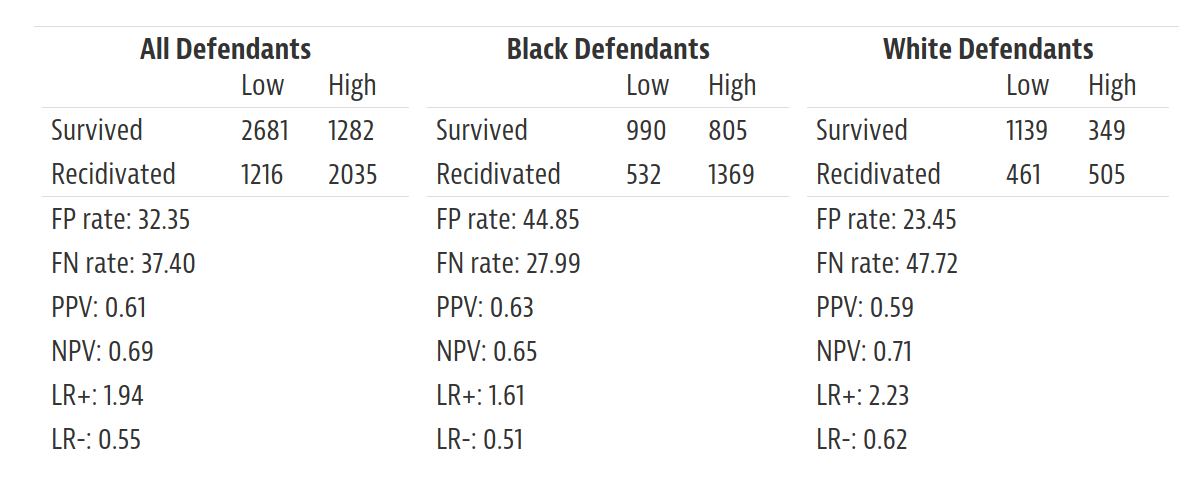
\includegraphics[width=4in]{chapters/figs/machine_bias_table.png}

The table summarizes results for all defendants and two subgroups:
defendants classified as White (``Caucasian'' in the original dataset)
and Black (``African-American''). For each group, the summary includes
several metrics, including:

\begin{itemize}

\item
  FP rate: false positive rate
\item
  FN rate: false negative rate
\item
  PPV: positive predictive value
\item
  NPV: negative predictive value
\item
  LR+: positive likelihood ratio
\item
  LR-: negative likelihood ratio
\end{itemize}

I will explain what these metrics mean and how to compute them, and
we'll replicate the results in this table. But first let's examine the
data and compute some recoded variables. The following function displays
the values in a Series and the number of times each value appears.

\begin{lstlisting}[]
def values(series):
    """Count the values and sort.
    
    series: pd.Series
    
    returns: series mapping from values to frequencies
    """
    return series.value_counts(dropna=False).sort_index()
\end{lstlisting}

Here are the values of \passthrough{\lstinline!decile\_score!}, which is
the output of the COMPAS algorithm. \passthrough{\lstinline!1!} is the
lowest risk category; \passthrough{\lstinline!10!} is the highest.

\begin{lstlisting}[]
values(cp['decile_score'])
\end{lstlisting}

\begin{tabular}{lr}
\midrule
{} &  decile\_score \\
\midrule
1  &          1440 \\
2  &           941 \\
3  &           747 \\
4  &           769 \\
5  &           681 \\
6  &           641 \\
7  &           592 \\
8  &           512 \\
9  &           508 \\
10 &           383 \\
\midrule
\end{tabular}

It's important to note that COMPAS is not a binary classifier; that is,
it does not predict that a defendant will or will not recidivate.
Rather, it gives each defendant a score that is intended to reflect the
risk that they will recidivate.

In order to evaluate the performance of COMPAS, the authors of the
ProPublica article chose a threshold, \passthrough{\lstinline!4!}, and
defined decile scores at or below the threshold to be ``low risk'', and
scores above the threshold to be ``high risk''. Their choice of the
threshold is arbitrary. Later, we will see what happens with other
choices, but we'll start by replicating the original analysis.

We'll create a Boolean \passthrough{\lstinline!Series!} called
\passthrough{\lstinline!high\_risk!} that's
\passthrough{\lstinline!True!} for respondents with a decile score
greater than 4.

\begin{lstlisting}[]
high_risk = (cp['decile_score'] > 4)
high_risk.name = 'HighRisk'
values(high_risk)
\end{lstlisting}

\begin{tabular}{lr}
\midrule
{} &  HighRisk \\
\midrule
False &      3897 \\
True  &      3317 \\
\midrule
\end{tabular}

The column \passthrough{\lstinline!two\_year\_recid!} indicates whether
a defendant was charged with another crime during a two year period
after the original charge when they were not in a correctional facility.

\begin{lstlisting}[]
values(cp['two_year_recid'])
\end{lstlisting}

\begin{tabular}{lr}
\midrule
{} &  two\_year\_recid \\
\midrule
0 &            3963 \\
1 &            3251 \\
\midrule
\end{tabular}

Let's create another \passthrough{\lstinline!Series!}, called
\passthrough{\lstinline!new\_charge!}, that is
\passthrough{\lstinline!True!} for defendants who were charged with
another crime within two years.

\begin{lstlisting}[]
new_charge = (cp['two_year_recid'] == 1)
new_charge.name = 'NewCharge'
values(new_charge)
\end{lstlisting}

\begin{tabular}{lr}
\midrule
{} &  NewCharge \\
\midrule
False &       3963 \\
True  &       3251 \\
\midrule
\end{tabular}

If we make a cross-tabulation of \passthrough{\lstinline!new\_charge!}
and \passthrough{\lstinline!high\_risk!}, the result is a DataFrame that
indicates how many defendants are in each of four groups:

\begin{lstlisting}[]
pd.crosstab(new_charge, high_risk)
\end{lstlisting}

\begin{tabular}{lrr}
\midrule
HighRisk &  False &  True  \\
NewCharge &        &        \\
\midrule
False     &   2681 &   1282 \\
True      &   1216 &   2035 \\
\midrule
\end{tabular}

This table is called a \textbf{confusion matrix} or error matrix.
Reading from left to right and top to bottom, the elements of the matrix
show the number of respondents who were:

\begin{itemize}
\item
  Classified as low risk and not charged with a new crime: there were
  2681 \textbf{true negatives}; that is, cases where the test was
  negative (not high risk) and the prediction turned out to be correct
  (no new charge).
\item
  High risk and not charged: there were 1282 \textbf{false positives},
  cases where the test was positive and the prediction was incorrect.
\item
  Low risk and charged: there were 1216 \textbf{false negatives}, cases
  where the test was negative (low risk) and the prediction was
  incorrect (the defendant was charged with a new crime).
\item
  High risk and charged: there were 2035 \textbf{true positives}, cases
  where the test was positive and the prediction was correct.
\end{itemize}

The values in this matrix are consistent with the values in the
ProPublica article, so we can confirm that we are reading the data and
replicating their analysis correctly.

Now let's check the confusion matrices for White and Black defendants.
Here are the values of \passthrough{\lstinline!race!}:

\begin{lstlisting}[]
values(cp['race'])
\end{lstlisting}

\begin{tabular}{lr}
\midrule
{} &  race \\
\midrule
African-American &  3696 \\
Asian            &    32 \\
Caucasian        &  2454 \\
Hispanic         &   637 \\
Native American  &    18 \\
Other            &   377 \\
\midrule
\end{tabular}

Here's a Boolean \passthrough{\lstinline!Series!} that's true for White
defendants.

\begin{lstlisting}[]
white = (cp['race'] == 'Caucasian')
white.name = 'white'
values(white)
\end{lstlisting}

\begin{tabular}{lr}
\midrule
{} &  white \\
\midrule
False &   4760 \\
True  &   2454 \\
\midrule
\end{tabular}

And here's the confusion matrix for White defendants.

\begin{lstlisting}[]
pd.crosstab(new_charge[white], high_risk[white])
\end{lstlisting}

\begin{tabular}{lrr}
\midrule
HighRisk &  False &  True  \\
NewCharge &        &        \\
\midrule
False     &   1139 &    349 \\
True      &    461 &    505 \\
\midrule
\end{tabular}

\passthrough{\lstinline!black!} is a Boolean Series that is
\passthrough{\lstinline!True!} for Black defendants.

\begin{lstlisting}[]
black = (cp['race'] == 'African-American')
black.name = 'black'
values(black)
\end{lstlisting}

\begin{tabular}{lr}
\midrule
{} &  black \\
\midrule
False &   3518 \\
True  &   3696 \\
\midrule
\end{tabular}

And here is the confusion matrix for Black defendants.

\begin{lstlisting}[]
pd.crosstab(new_charge[black], high_risk[black])
\end{lstlisting}

\begin{tabular}{lrr}
\midrule
HighRisk &  False &  True  \\
NewCharge &        &        \\
\midrule
False     &    990 &    805 \\
True      &    532 &   1369 \\
\midrule
\end{tabular}

All of these results are consistent with the ProPublica article.
However, before we go on, I want to address an important issue with this
dataset: data bias.

\hypertarget{data-bias}{%
\section{Data Bias}\label{data-bias}}

Systems like COMPAS are trying to predict whether a defendant will
\emph{commit} another crime if released. But the dataset reports whether
a defendant was \emph{charged} with another crime.

Not everyone who commits a crime gets charged (not even close). The
probability of getting charged for a particular crime depends on the
type of crime and location; the presence of witnesses and their
willingness to work with police; the decisions of police about where to
patrol, what crimes to investigate, and who to arrest; and decisions of
prosecutors about who to charge.

It is likely that every one of these factors depends on the race of the
defendant. In this dataset, the prevalence of \emph{new charges} is
higher for Black defendants, but that doesn't necessarily mean that the
prevalence of \emph{new crimes} is higher.

If the dataset is affected by racial bias in the probability of being
charged, prediction algorithms like COMPAS will be biased, too. In
discussions of whether and how these systems should be used in the
criminal justice system, this is an important issue.

However, I am going to put it aside \emph{for now} in order to focus on
understanding the arguments posed in the ProPublica article and the
metrics they are based on. For the rest of this chapter I will take the
``recidivism rates'' in the dataset at face value; but I will try to be
clear about that they mean (and don't mean).

\hypertarget{arranging-the-confusion-matrix}{%
\section{Arranging the confusion
matrix}\label{arranging-the-confusion-matrix}}

In the previous section I arranged the confusion matrix to be consistent
with the ProPublica article, to make it easy to check for consistency.

In general, there are many ways to arrange a confusion matrix: you can
put the predictions along the columns and the actual conditions along
the rows, or the other way around, and you can sort the rows and columns
in either order.

There is no universal standard arrangement, but the most common one
looks like this:

\begin{longtable}[]{@{}
  >{\raggedright\arraybackslash}p{(\columnwidth - 4\tabcolsep) * \real{0.3043}}
  >{\raggedright\arraybackslash}p{(\columnwidth - 4\tabcolsep) * \real{0.3478}}
  >{\raggedright\arraybackslash}p{(\columnwidth - 4\tabcolsep) * \real{0.3478}}@{}}
\midrule()
\begin{minipage}[b]{\linewidth}\raggedright
\end{minipage} & \begin{minipage}[b]{\linewidth}\raggedright
\textbf{Predicted positive}
\end{minipage} & \begin{minipage}[b]{\linewidth}\raggedright
\textbf{Predicted negative}
\end{minipage} \\
\midrule()
\endhead
\textbf{Actual positive} & True positive (TP) & False negative (FN) \\
\textbf{Actual negative} & False positive (FP) & True negative (TN) \\
\midrule()
\end{longtable}

In this arrangement:

\begin{itemize}
\item
  The actual conditions are down the rows.
\item
  The predictions are across the columns.
\item
  The rows and columns are sorted so true positives are in the upper
  left and true negatives are in the lower right.
\end{itemize}

In the context of the ProPublica article:

\begin{itemize}
\item
  ``Predicted positive'' means the defendant is classified as high risk.
\item
  ``Predicted negative'' means low risk.
\item
  ``Actual positive'' means the defendant was charged with a new crime
  (recidivated).
\item
  ``Actual negative'' means they were not charged (survived).
\end{itemize}

Going forward, we'll present confusion matrices in this format.

Here is the confusion matrix for all defendants.

\begin{lstlisting}[]
matrix_all = make_matrix(cp)
matrix_all
\end{lstlisting}

\begin{tabular}{lrr}
\midrule
{} &  Pred Positive &  Pred Negative \\
Actual   &                &                \\
\midrule
Positive &           2035 &           1216 \\
Negative &           1282 &           2681 \\
\midrule
\end{tabular}

\hypertarget{accuracy}{%
\section{Accuracy}\label{accuracy}}

Based on these results, how accurate is COMPAS as a binary classifier?
Well, it turns out that there are a \emph{lot} of ways to answer that
question. One of the simplest is overall \textbf{accuracy}, which is the
fraction (or percentage) of correct predictions. To compute accuracy, it
is convenient to extract from the confusion matrix the number of true
positives, false negatives, false positives, and true negatives.

\begin{lstlisting}[]
tp, fn, fp, tn = matrix_all.to_numpy().flatten()
\end{lstlisting}

The number of true predictions is \passthrough{\lstinline!tp + tn!}. The
number of false predictions is \passthrough{\lstinline!fp + fn!}. So we
can compute the fraction of true predictions like this:

\begin{lstlisting}[]
def percent(x, y):
    """Compute the percentage `x/(x+y)*100`."""
    return x / (x+y) * 100
\end{lstlisting}

\begin{lstlisting}[]
accuracy = percent(tp + tn, fp + fn)
accuracy
(@\dashfill@)
@@@65.37288605489326@@@
\end{lstlisting}

As a way to evaluate a binary classifier, accuracy does not distinguish
between true positives and true negatives, or false positives and false
negatives.

But it is often important to make these distinctions, because the
benefits of true predictions and true negatives might be different, and
the costs of false positives and false negatives might be different.

\hypertarget{predictive-value}{%
\section{Predictive Value}\label{predictive-value}}

One way to make these distinctions is to compute the ``predictive
value'' of positive and negative tests:

\begin{itemize}
\item
  \textbf{Positive predictive value (PPV)} is the fraction of positive
  tests that are correct.
\item
  \textbf{Negative predictive value (NPV)} is the fraction of negative
  tests that are correct.
\end{itemize}

In this example, PPV is the fraction of high risk defendants who were
charged with a new crime. NPV is the fraction of low risk defendants who
``survived'' a two year period without being charged.

The following function takes a confusion matrix and computes these
metrics.

\begin{lstlisting}[]
def predictive_value(m):
    """Compute positive and negative predictive value.
    
    m: confusion matrix
    """
    tp, fn, fp, tn = m.to_numpy().flatten()
    ppv = percent(tp, fp)
    npv = percent(tn, fn)
    return ppv, npv
\end{lstlisting}

Here are the predictive values for all defendants.

\begin{lstlisting}[]
ppv, npv = predictive_value(matrix_all)
ppv, npv
(@\dashfill@)
@@@(61.350618028338864, 68.79651013600206)@@@
\end{lstlisting}

Among all defendants, a positive test is correct about 61\% of the time;
a negative test result is correct about 69\% of the time.

\hypertarget{sensitivity-and-specificity}{%
\section{Sensitivity and
Specificity}\label{sensitivity-and-specificity}}

Another way to characterize the accuracy of a test is to compute

\begin{itemize}
\item
  \textbf{Sensitivity}, which is the probability of predicting correctly
  when the condition is present, and
\item
  \textbf{Specificity}, which is the probability of predicting correctly
  when the condition is absent.
\end{itemize}

A test is ``sensitive'' if it detects the positive condition. In this
example, sensitivity is the fraction of recidivists who were correctly
classified as high risk.

A test is ``specific'' if it identifies the negative condition. In this
example, specificity is the fraction of non-recidivists who were
correctly classified as low risk.

The following function takes a confusion matrix and computes sensitivity
and specificity.

\begin{lstlisting}[]
def sens_spec(m):
    """Compute sensitivity and specificity.
    
    m: confusion matrix
    """
    tp, fn, fp, tn = m.to_numpy().flatten()
    sens = percent(tp, fn)
    spec = percent(tn, fp)
    return sens, spec
\end{lstlisting}

Here are sensitivity and specificity for all defendants.

\begin{lstlisting}[]
sens, spec = sens_spec(matrix_all)
sens, spec
(@\dashfill@)
@@@(62.59612426945556, 67.65076961897553)@@@
\end{lstlisting}

If we evaluate COMPAS as a binary classifier, it is a little more
specific than sensitive:

\begin{itemize}
\item
  About 63\% of the recidivists were classified as high risk.
\item
  About 68\% of the non-recidivists were classified as low risk.
\end{itemize}

It can be hard to keep all of these metrics straight, especially when
you are learning about them for the first time. The following table
might help:

\begin{longtable}[]{@{}
  >{\raggedright\arraybackslash}p{(\columnwidth - 8\tabcolsep) * \real{0.1807}}
  >{\raggedright\arraybackslash}p{(\columnwidth - 8\tabcolsep) * \real{0.2229}}
  >{\raggedright\arraybackslash}p{(\columnwidth - 8\tabcolsep) * \real{0.2229}}
  >{\raggedright\arraybackslash}p{(\columnwidth - 8\tabcolsep) * \real{0.1928}}
  >{\raggedright\arraybackslash}p{(\columnwidth - 8\tabcolsep) * \real{0.1807}}@{}}
\midrule()
\begin{minipage}[b]{\linewidth}\raggedright
\end{minipage} & \begin{minipage}[b]{\linewidth}\raggedright
\textbf{Pred positive (PP)}
\end{minipage} & \begin{minipage}[b]{\linewidth}\raggedright
\textbf{Pred negative (PN)}
\end{minipage} & \begin{minipage}[b]{\linewidth}\raggedright
\end{minipage} & \begin{minipage}[b]{\linewidth}\raggedright
\end{minipage} \\
\midrule()
\endhead
\textbf{Actual positive (P)} & True positive (TP) & False negative (FN)
& Sensitivity = TP / P & FN rate = FN / P \\
\textbf{Actual negative (N)} & False positive (FP) & True negative (TN)
& FP rate = FP / N & Specificity = TN / N \\
Prevalence = P / (P + N) & PPV = TP / PP & NPV = TN / PN & & Acc = (TP +
TN) / (P + N) \\
\midrule()
\end{longtable}

PPV and sensitivity are similar in the sense that they both have true
positives in the numerator. The difference is the denominator:

\begin{itemize}
\item
  PPV is the ratio of true positives to all positive tests. So it
  answers the question, ``Of all positive tests, how many are correct?''
\item
  Sensitivity is the ratio of true positives to all positive conditions.
  So it answers the question ``Of all positive conditions, how many are
  detected?''
\end{itemize}

Similarly, NPV and sensitivity both have true negatives in the
numerator, but:

\begin{itemize}
\item
  NPV is the ratio of true negatives to all negative tests. It answers,
  ``Of all negative tests, how many are correct?''
\item
  Specificity is the ratio of true negatives to all negative conditions.
  It answers, ``Of all negative conditions, how many are classified
  correctly?''
\end{itemize}

\hypertarget{false-positive-and-negative-rates}{%
\section{False Positive and Negative
Rates}\label{false-positive-and-negative-rates}}

The ProPublica article reports PPV and NPV, but instead of sensitivity
and specificity, it reports their complements:

\begin{itemize}
\item
  \textbf{False positive rate}, which is the ratio of false positives to
  all negative conditions. It answers, ``Of all negative conditions, how
  many are misclassified?''
\item
  \textbf{False negative rate}, which is the ratio of false negatives to
  all positive conditions. It answers, ``Of all positive conditions, how
  many are misclassified?''
\end{itemize}

In this example:

\begin{itemize}
\item
  The false positive rate is the fraction of non-recidivists who were
  classified as high risk.
\item
  The false negative rate is the fraction of recidivists who were
  classified as low risk.
\end{itemize}

The following function takes a confusion matrix and computes false
positive and false negative rates.

\begin{lstlisting}[]
def error_rates(m):
    """Compute false positive and false negative rate.
    
    m: confusion matrix
    """
    tp, fn, fp, tn = m.to_numpy().flatten()
    fpr = percent(fp, tn)
    fnr = percent(fn, tp)
    return fpr, fnr
\end{lstlisting}

Here are the error rates for all defendants.

\begin{lstlisting}[]
fpr, fnr = error_rates(matrix_all)
fpr, fnr
(@\dashfill@)
@@@(32.349230381024476, 37.40387573054445)@@@
\end{lstlisting}

FPR is the complement of specificity, which means they have to add up to
100\%

\begin{lstlisting}[]
fpr + spec
(@\dashfill@)
@@@100.0@@@
\end{lstlisting}

And FNR is the complement of sensitivity.

\begin{lstlisting}[]
fnr + sens
(@\dashfill@)
@@@100.0@@@
\end{lstlisting}

So FPR and FNR are just another way of reporting sensitivity and
specificity. In general, I prefer sensitivity and specificity over FPN
and FNR because

\begin{itemize}
\item
  I think the positive framing is easier to interpret than the negative
  framing, and
\item
  I find it easier to remember what ``sensitivity'' and ``specificity''
  mean.
\end{itemize}

I think ``false positive rate'' and ``false negative rate'' are more
problematic. For example, ``false positive rate'' could just as easily
mean either

\begin{enumerate}
\def\labelenumi{\arabic{enumi}.}
\item
  The fraction of positive tests that are incorrect, or
\item
  The fraction of negative conditions that are misclassified.
\end{enumerate}

It is only a convention that the first is called the ``false discovery
rate'' and the second is called ``false positive rate''. I suspect I am
not the only one that gets them confused.

So, here's my recommendation: if you have the choice, generally use PPV,
NPV, sensitivity and specificity, and avoid the other metrics. However,
since the ProPublica article uses FPR and FNR, I will too. They also
report LR+ and LR-, but those are combinations of other metrics and not
relevant to the current discussion, so I will ignore them.

However, there is one other metric that I think is relevant and not
included in the ProPublica tables: \textbf{prevalence}, which is the
fraction of all cases where the condition is positive. In the example,
it's the fraction of defendants who recidivate. The following function
computes prevalence:

\begin{lstlisting}[]
def prevalence(m):
    """Compute prevalence.
    
    m: confusion matrix
    """
    tp, fn, fp, tn = m.to_numpy().flatten()
    prevalence = percent(tp+fn, tn+fp)
    return prevalence
\end{lstlisting}

Here's the prevalence for all defendants:

\begin{lstlisting}[]
prev = prevalence(matrix_all)
prev
(@\dashfill@)
@@@45.06515109509287@@@
\end{lstlisting}

About 45\% of the defendants in this dataset were charged with another
crime within two years of their release.

\hypertarget{all-metrics}{%
\section{All Metrics}\label{all-metrics}}

The following function takes a confusion matrix, computes all the
metrics, and puts them in a DataFrame.

\begin{lstlisting}[]
def compute_metrics(m, name=''):
    """Compute all metrics.
    
    m: confusion matrix
    
    returns: DataFrame
    """
    fpr, fnr = error_rates(m)
    ppv, npv = predictive_value(m)
    prev = prevalence(m)
    
    index = ['FP rate', 'FN rate', 'PPV', 'NPV', 'Prevalence']
    df = pd.DataFrame(index=index, columns=['Percent'])
    df.Percent = fpr, fnr, ppv, npv, prev
    df.index.name = name
    return df.round(1)
\end{lstlisting}

Here are the metrics for all defendants.

\begin{lstlisting}[]
compute_metrics(matrix_all, 'All defendants')
\end{lstlisting}

\begin{tabular}{lr}
\midrule
{} &  Percent \\
All defendants &          \\
\midrule
FP rate        &     32.3 \\
FN rate        &     37.4 \\
PPV            &     61.4 \\
NPV            &     68.8 \\
Prevalence     &     45.1 \\
\midrule
\end{tabular}

Comparing these results to the table from ProPublica, it looks like our
analysis agrees with theirs.

Here are the same metrics for Black defendants.

\begin{lstlisting}[]
compute_metrics(matrix_black, 'Black defendants')
\end{lstlisting}

\begin{tabular}{lr}
\midrule
{} &  Percent \\
Black defendants &          \\
\midrule
FP rate          &     44.8 \\
FN rate          &     28.0 \\
PPV              &     63.0 \\
NPV              &     65.0 \\
Prevalence       &     51.4 \\
\midrule
\end{tabular}

And for White defendants.

\begin{lstlisting}[]
compute_metrics(matrix_white, 'White defendants')
\end{lstlisting}

\begin{tabular}{lr}
\midrule
{} &  Percent \\
White defendants &          \\
\midrule
FP rate          &     23.5 \\
FN rate          &     47.7 \\
PPV              &     59.1 \\
NPV              &     71.2 \\
Prevalence       &     39.4 \\
\midrule
\end{tabular}

All of these results are consistent with those reported in the article,
including the headline results:

\begin{enumerate}
\def\labelenumi{\arabic{enumi}.}
\item
  The false positive rate for Black defendants is substantially higher
  than for White defendants (45\%, compared to 23\%).
\item
  The false negative rate for Black defendants is substantially lower
  (28\%, compared to 48\%).
\end{enumerate}

\begin{lstlisting}[]
error_rates(matrix_black)
(@\dashfill@)
@@@(44.84679665738162, 27.985270910047344)@@@
\end{lstlisting}

\begin{lstlisting}[]
error_rates(matrix_white)
(@\dashfill@)
@@@(23.45430107526882, 47.72256728778468)@@@
\end{lstlisting}

In other words:

\begin{itemize}
\item
  Of all people who \emph{will not} recidivate, Black defendants are
  more likely to be be classified as high risk and (if these
  classifications influence sentencing decisions) more likely to be sent
  to prison.
\item
  Of all people who \emph{will} recidivate, White defendants are more
  likely to be classified as low risk, and more likely to be released.
\end{itemize}

This seems clearly unfair.

However, it turns out that ``fair'' is complicated. After the ProPublica
article, the Washington Post published a response by Sam Corbett-Davies,
Emma Pierson, Avi Feller and Sharad Goel: ``A computer program used for
bail and sentencing decisions was labeled biased against blacks. It's
actually not that clear,'' at
\url{https://www.washingtonpost.com/news/monkey-cage/wp/2016/10/17/can-an-algorithm-be-racist-our-analysis-is-more-cautious-than-propublicas}.

I encourage you to read that article, and then read the next chapter,
where I will unpack their arguments and replicate their analysis.

